\chapter{Topologically Optimal Structures}
\label{chap:a30structures}

\noindent
This appendix complements \cref{sec:64results}.
It contains visualizations of the topologically optimal structures
in the 2D L-shape and the 3D scenarios in
\cref{fig:topoOptStructure2DLShape} and \cref{fig:topoOptStructure3D},
respectively.
In addition, we report details of the corresponding optimization runs
in \cref{tbl:topoOptResultsDetailed} and
information about the employed spatially adaptive sparse grids in
\cref{tbl:topoOptResultsModels}.
The runtimes were measured on a shared memory computer
with 4x Intel Xeon E7-8880v3 (72 cores, 144 threads).

\begin{figure}
  \subcaptionbox{%
    2D cross%
  }[72mm]{%
    % id = 651
    \includegraphics{topoOptStructure2D_2}%
  }%
  \hfill%
  \subcaptionbox{%
    2D framed cross%
  }[72mm]{%
    % id = 653
    \includegraphics{topoOptStructure2D_4}%
  }%
  \\[2mm]%
  \subcaptionbox{%
    2D sheared cross%
  }[72mm]{%
    % id = 655
    \includegraphics{topoOptStructure2D_6}%
  }%
  \hfill%
  \subcaptionbox{%
    2D sheared framed cross%
  }[72mm]{%
    % id = 657
    \includegraphics{topoOptStructure2D_8}%
  }%
  \caption[Optimal structures in the 2D L-shape scenario]{%
    Topologically optimal structures in the 2D L-shape scenario
    for different micro-cell models using cubic B-splines
    (spatially adaptive grids with around \num{10000} points).
    The colors indicate the length of the displacement,
    where dark regions correspond to weak displacements and
    bright regions to strong displacements.
    The color map is the same as in
    \cref{fig:topoOptStructure2DCantilever}.
    More details can be found in \cref{tbl:topoOptResultsDetailed}.%
  }%
  \label{fig:topoOptStructure2DLShape}%
\end{figure}

\begin{figure}
  % To generate the plots:
  % 1.  python3 image.py --id XXX --3d-threshold 0.01 --density --save
  % 2.  python3 3d_model.py --id XXX
  % 3.  Open resulting sims/test.png in GIMP
  % 4.  Colours -> Hue-Saturation -> reduce saturation by 50% (i.e., -50%)
  % 5.  Colours -> Brightness-Contrast
  %             -> increase brightness and contrast each by 60%
  % 6.  Image -> Scale Image -> scale to 66.67%
  % 7.  Set background color to e5eef5 (should be mittelblau!10)
  % 8.  Layer -> Transparency -> Remove Alpha Channel
  % 9.  Image -> Autocrop Image
  % 10. Export as PNG
  \newcommand*{\myscale}{0.19}%
  \subcaptionbox{%
    3D cantilever, 3D cross%
  }[72mm]{%
    % id = 658
    \includegraphics[scale=\myscale]{topoOptStructure658}%
  }%
  \hfill%
  \subcaptionbox{%
    3D cantilever, 3D sheared cross%
  }[72mm]{%
    % id = 660
    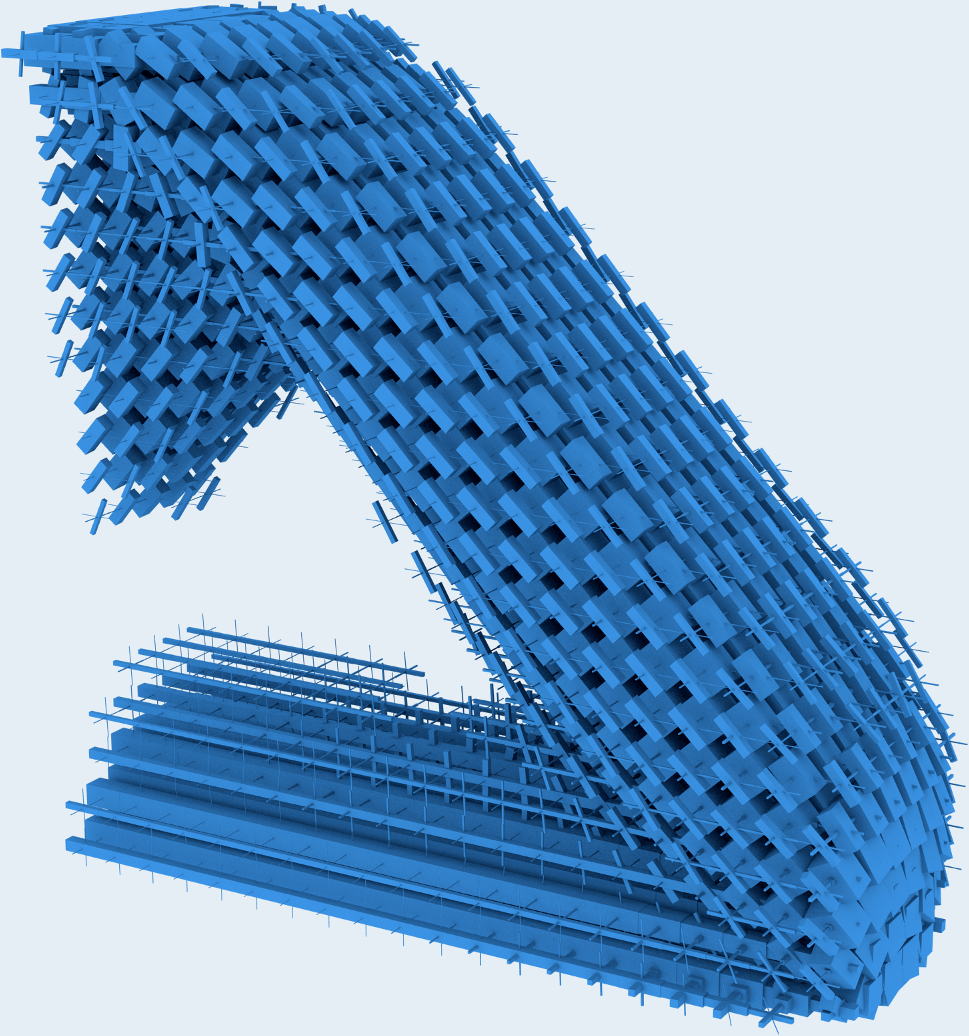
\includegraphics[scale=\myscale]{topoOptStructure660}%
  }%
  \\[2mm]%
  \begin{tikzpicture}
    \node[anchor=south west] at (0mm,61mm) {%
      \includegraphics[scale=\myscale]{topoOptStructure659}%
    };
    \node[anchor=south west] at (0mm,0mm) {%
      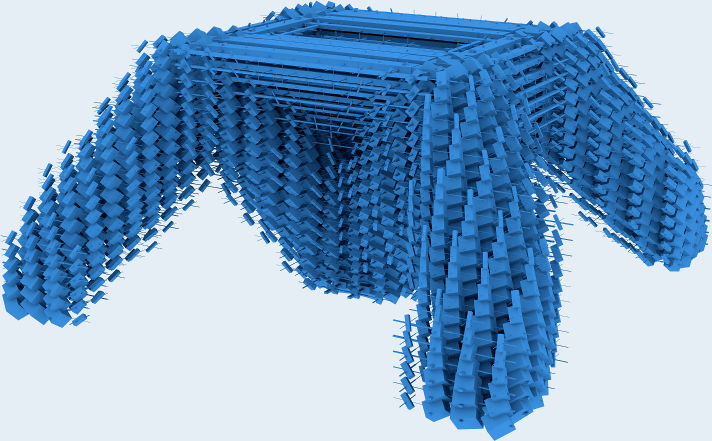
\includegraphics[scale=\myscale]{topoOptStructure661}%
    };
    \node[anchor=south west,text width=50mm] at (-1mm,66mm) {%
      \subcaption{3D center-load, 3D cross}%
    };
    \node[anchor=south west,text width=60mm] at (-8mm,5mm) {%
      \subcaption{3D center-load, 3D sheared cross}%
    };
  \end{tikzpicture}
  \hspace*{6mm}
  \caption[Optimal structures in the 3D scenarios]{%
    Topologically optimal structures in the
    3D cantilever and center-load scenarios
    for different micro-cell models using cubic B-splines
    (spatially adaptive grids with around \num{10000} points).
    More details can be found in \cref{tbl:topoOptResultsDetailed}.%
  }%
  \label{fig:topoOptStructure3D}%
\end{figure}

\begin{table}
  \sisetup{retain-zero-exponent=true}%
  \newcommand*{\cece}[1]{\multicolumn{1}{c}{#1}}%
  \newcommand*{\trcmp}{\compliance[\opt,\ast]}%
  \newcommand*{\apcmp}{\complianceintp[\opt,\ast]}%
  \newcommand*{\iic}{\multirow{-4}{*}{2D cantilever}}%
  \newcommand*{\iil}{\multirow{-4}{*}{2D L-shape}}%
  \newcommand*{\iiic}{\multirow{-2}{*}{3D cantilever}}%
  \newcommand*{\iiicl}{\multirow{-2}{*}{3D center-load}}%
  \setnumberoftableheaderrows{1}%
  \begin{tabular}{%
    >{\kern\tabcolsep}=l+l<{\kern5mm}+r+c+c+l+r<{\kern\tabcolsep}%
  }
    \toprulec
    \headerrow
    Scenario& Model& \#Iter.& $\trcmp$& $\apcmp$& \cece{O.-i. gap}& Runtime\\
    \midrulec
    % id = 650,652,654,656
    &         2D-C&      547& 74.974&   74.974&   \num{3.67e-5}&    \hms{;5}\\
    &         2D-FC&     249& 70.816&   69.409&   \num{1.41e0}&     \hms{;14}\\
    &         2D-SC&    2196& 67.809&   67.804&   \num{5.21e-3}&    \hms{1;6}\\
    \iic&     2D-SFC&    749& 68.602&   65.201&   \num{3.40e0}&     \hms{;15}\\
    \midrulec
    % id = 651,653,655,657
    &         2D-C&      289& 183.68&   183.68&   \num{9.06e-5}&    \hms{;3}\\
    &         2D-FC&     602& 177.51&   174.49&   \num{3.02e0}&     \hms{;17}\\
    &         2D-SC&    1609& 169.60&   169.60&   \num{7.33e-3}&    \hms{;33}\\
    \iil&     2D-SFC&    574& 174.55&   158.19&   \num{1.64e1}&     \hms{;8}\\
    \midrulec
    % id = 658,660
    &         3D-C&       39& 247.60&   247.49&   \num{1.13e-1}&    \hms{;10}\\
    \iiic&    3D-SC&     608& 162.59&   159.33&   \num{3.25e0}&     \hms{3;17}\\
    \midrulec
    % id = 659,661
    &         3D-C&       35& 169.27&   169.27&   \num{3.31e-3}&    \hms{;4}\\
    \iiicl&   3D-SC&    1026& 46.171&   45.571&   \num{6.00e-1}&    \hms{2;25}\\
    \bottomrulec
  \end{tabular}
  \caption[Detailed information about topology optimization runs]{%
    Detailed information about the optimization runs corresponding to
    \cref{tbl:topoOptResultsModels} and
    \cref{%
      fig:topoOptStructure2DCantilever,%
      fig:topoOptStructure2DLShape,%
      fig:topoOptStructure3D%
    }, which employs cubic B-splines ($p = 3$) on the spatially
    adaptive grids listed in \cref{tbl:topoOptResultsModels}.
    From left to right, the columns contain
    the optimization scenario,
    the micro-cell model,
    the number of optimization iterations,
    the actual compliance value
    $\trcmp := \compliance(\mcpoptappr{1}, \dotsc, \mcpoptappr{M})$,
    the approximated compliance value
    $\apcmp := \complianceintp(\mcpoptappr{1}, \dotsc, \mcpoptappr{M})$
    as reported by the optimizer,
    the optimality-interpolation gaps $\abs{\trcmp - \apcmp}$, and
    the runtime of the online phase
    (without the time to generate the sparse grid data).%
  }%
  \label{tbl:topoOptResultsDetailed}%
\end{table}

\begin{table}
  \sisetup{retain-zero-exponent=true}%
  \newcommand*{\cece}[1]{\multicolumn{1}{c}{#1}}%
  \setnumberoftableheaderrows{1}%
  \begin{tabular}{%
    >{\kern\tabcolsep}=l<{\kern5mm}+c+r+l+l+c<{\kern\tabcolsep}%
  }
    \toprulec
    \headerrow
    Model&  $d$& \#Points& \cece{Threshold}& \cece{Rel. err.}& Eval. time\\
    \midrulec
    % cross-sisc-conv-tol2.15443e-05-lb0.01-ub0.99-cholesky-hier-bspl3
    % Homogenization.generateShearedCrossExact
    2D-C&   2&   10197&    \num{2.15e-5}&    \num{2.24e-5}&    \SI{6.96}{\second}\\
    % framed-cross-sga16-conv-tol0.794328-lb0.01-ub0.99-cholesky-hier-bspl3
    % Homogenization.generateFramedCross
    2D-FC&  4&   10502&    \num{7.94e-1}&    \num{1.81e-2}&    \SI{7.45}{\second}\\
    % sheared-cross-sisc-conv-tol0.00464159-lb0.01,0.15-ub0.99,0.85-cholesky-hier-bspl3
    % Homogenization.generateShearedCrossExact
    2D-SC&  3&   10723&    \num{4.64e-3}&    \num{1.49e-3}&    \SI{8.72}{\second}\\
    % sheared-framed-cross-sga16-conv-tol5.01187-lb0.01,0.15-ub0.99,0.85-cholesky-hier-bspl3
    % Homogenization.generateShearedFramedCross
    2D-SFC& 5&   10694&    \num{5.01e0}&     \num{4.82e-2}&    \SI{7.45}{\second}\\
    \midrulec
    % cross-3d-sga16-conv-tol0.0794328-lb0.01-ub0.99-cholesky-hier-bspl3
    % Homogenization.generateCross3DExact
    3D-C&   3&    9207&    \num{7.94e-2}&    \num{3.18e-3}&    \SI{33.5}{\second}\\
    % sheared-cross-3d-sga16-conv-tol5.01187-lb0.01,0.15-ub0.99,0.85-cholesky-hier-bspl3
    % Homogenization.generateShearedCross3DExact
    3D-SC&  5&   15389&    \num{5.01e0}&     \num{4.95e-2}&    \SI{40.0}{\second}\\
    \bottomrulec
  \end{tabular}
  \caption[Detailed information about spatially adaptive sparse grids]{%
    Detailed information about the spatially adaptive sparse grids used for
    \cref{tbl:topoOptResultsModels,tbl:topoOptResultsDetailed} and
    \cref{%
      fig:topoOptStructure2DCantilever,%
      fig:topoOptStructure2DLShape,%
      fig:topoOptStructure3D%
    }.
    The columns correspond to
    the micro-cell model,
    the number $d$ of micro-cell parameters,
    the number of sparse grid points,
    the threshold $\refinetol$ used in the grid generation algorithm,
    the relative $\Ltwo$ spectral interpolation error
    $
      \normLtwoscaled{
        \vphantom{\big(}
        \norm[2]{\etensor({\cdot}) - \etensorcholintp({\cdot})}
      }
      /
      \normLtwoscaled{
        \vphantom{\big(}
        \norm[2]{\etensor({\cdot})}
      }
    $, and the
    time needed to evaluate the elasticity tensor $\etensor(\vgp{k})$
    at a single grid point $\vgp{k}$.%
  }%
  \label{tbl:topoOptModels}%
\end{table}

\cleardoublepage
